\chapter{Cognitive Radio: A Brief Overview}

\section{Introduction}

Technology is advancing rapidly, especially
in the filed of wireless communications. New communication devices and signal architectures are invented
every day, and therfore there is a dire need for higher data rates. However, the
radio frequency (RF) spectrum is limited, and not all the devices can be
allocated spectrum with the present allocation schemes. A dynamic spectrum
allocation has to be introduced to accomodate new technologies, and use the
spectrum efficiently. This report discusses a possible solution to the problem
of spectrum sharing - Cognitive Radio. Chapter $1$ discusses the basics of
Cognitive Radio, its requirements and the challenges. A deeper insight into
methods of Spectrum Sharing (Interweave and Underlay) is given in Chapters $2$
and $3$.

\section{Radio Spectrum}
The radio spectrum is a limited natural resource\cite{haykin}. This spectrum is
divided into frequency bands, each for a particular service, and certain technologies.
Frequency allocation is decided by the International Telecommunication Union
(ITU), an agency of the United Nations, at the international level, and national
regulatory authorities at the national levels\cite{doyle}. Frequency assignment
is done at the national level, wherein subdivisions of the spectrum are assigned to
specific parties licensed to use them. This static allocation of the spectrum
leads to inefficiency in the spectrum usage. Interference Protection and Dynamic
Spectrum Access are very important for efficient spectrum usage.

\subsection{Interference Protection}
\cite{fcc1} states that interference protection is central to effective spectrum
management. RF devices are designed and operated based on interference
regulations and protocols. If the standards for interference protection are not
met, it can lead to ineffective communication. Interference protection
agreements are negotiated and formulated based on the allowed in-band power and
admissible out-of-band emissions. The problem with these regulations is that
they have to be updated regularly to meet the requirements of new technologies,
methods of transmissions and also environmental changes. The first major concern
is the sudden increase in RF devices sharing the spectrum, and their demand.
Mobile phones, TV remotes, electronic doors, automatic lights, WiFi, Bluetooth,
smart vehicles, radios are only few of the many RF devices that have to share
the spectrum on a daily basis, and a static interference protection paradigm
cannot set the standards of communication. Another major problem is the variety
of signal architectures and modulation types utilized today, compared to a few
years back. Even a single device uses multiple architectures to communicate.
This further supports the fact that a static protection paradigm is not
sufficient.

\subsection{Dynamic Spectrum Access}
The static allocation of radio spectrum results in its underutilization. The
frequency bands vary in usage - some are heavily used, while some are partially
occupied, and the rest are mostly unoccupied for large periods of
time\cite{haykin}. This results in spectrum holes. \cite{kolodzy} defines a spectrum
hole as a \textit{``band of frequencies assigned to a licensed user, but, at a particular time and
specific geographic location, the band is not being utilized by that
user.''} This can be depicted from figure \ref{fig:specholes}. 
\begin{figure}[h]
\centering
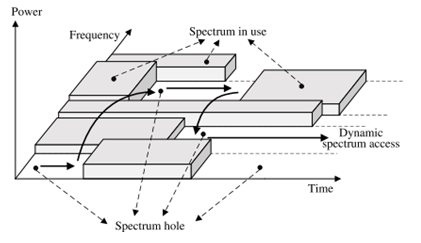
\includegraphics[keepaspectratio,scale=0.8]{images/spectral_holes.PNG}
\caption{Spectral Holes\cite{moghaddam}}
\label{fig:specholes}
\end{figure}
Spectrum Sensing provides a way to sense these spectral holes, and utilize them,
thereby increasing efficiency of spectrum usage. This, however requires a Dynamic Spectrum Access scheme, in which the non-licensed users
utilize the spectrum, when they sense it is not being utilized by the licensed
users.


\section{Cognitive Radio}
The term ``Cognitive Radio'' was first coined by Mitola and Maguire, in $1999$,
in an article they wrote together\cite{mitola}. The Cognitive Radio (CR) is
described as an intelligent radio, which understands its surroundings and can adapt its
communication accordingly. The Federal Communications Commission (FCC) defines a
CR as \textit{``a radio or system that senses its operational electromagnetic
environment and can dynamically and autonomously adjust its radio operating
parameters to modify system operation, such as maximize throughput, mitigate
interference, facilitate interoperability and access secondary
markets.''}\cite{fcc2} In simpler words, it is a smart radio, that can sense and
understand the channel characteristics, the transmission properties, the interference policies and
regulations and other operating restrictions, and then adapt to the best
communication strategy based on its own capabilities.

\subsection{The Cognitive Cycle}
The three main operations of a cognitive radio are \textit{``observe, decide
and act''}\cite{mitola} as shown in figure \ref{fig:cogcycle}.

\begin{figure}[h]
	\centering
	\includestandalone[keepaspectratio,scale=0.65]{images/fig_cogcycle}
	\caption{The Cognitive Cycle}
	\label{fig:cogcycle}
\end{figure}

The \textit{observe} step refers to the cognitive radio sensing the channel
parameters, and the presence of a licensed user, and the licensed user's
transmission characteristics. Based on these observations, the cognitive radio
has to \textit{decide} whether or not to allow the non-licensed user to
communicate. It has to calculate the allowed interference levels, power levels,
and duration of transmission for the non-licensed user in the given time frame.
These decisions are passed on to the \textit{act} phase, where the radio
reconfigures itself, to satisfy its decisions. This is a continuous cyclic
process, wherein the radio has to reconfigure itself dynamically, for any change
in operating or transmitting characteristics. This dynamic reconfigurability of
the CR helps increase the spectrum utility.

\subsection{Spectrum Sensing}
There are two types of users, namely primary and secondary users. Primary users,
or licensed users, pay for a particular band of frequencies, and utilize it for
their services. Secondary users, or non-licensed users, tend to use the licensed
spectrum whenever the primary user is not transmitting, or without interference
to the primary user. To maintain Quality of Service at the primary user side,
i.e no loss of data, and permissible interference, the CR should be able to
sense when a primary user is communicating, and the transmission parameters
being utilized. This process, called Spectrum Sensing, is the core of Cognitive
Radio. \cite{doyle} states that sensing in CR systems can be classified into two
ways - non-cooperative sensing and cooperative sensing.

\subsubsection{Non-Cooperative Sensing}
In a system employing non-cooperative sensing, each radio acts individually,
sensing its environment for primary transmissions and relaying that information
to the secondary users in its range. The main problem which arises in this
method is the hidden node problem, i.e a transmitter can be near the CR but not
be detected, due to fading in the sensing signal. This leads to the decision
that the spectrum is unoccupied, when it is actually occupied. Another problem
is the time taken to sense is very high in this case, as each node acts for
itself. So, cooperative sensing is suggested as a means to overcome these
problems.

\subsubsection{Cooperative Sensing}
Cooperative sensing employs a network of nodes sensing the spectrum together,
and relaying information among one another. The \textit{Centralized} approach
consists of a central node, and a network of nodes around it. This network
senses the spectrum, and relays its decisions back to the central node, which
processes the information and makes a decision as to whether the spectrum is
occupied or not. This information is then passed back to the nodes. Another
approach is the \textit{Distributed} approach, where there is no central node,
but the network of nodes share information amongst one another and make
decisions based on their requirements. The cooperative sensing approach
overcomes the hidden node problem, as though the transmitter may not be sensed
by one node, it would be sensed by another node in the network. The time
required for detection of primary user considerably reduces, due to
collaboration of all the nodes.

\subsection{Spectrum Sharing Approaches}
Once the CR has sensed the spectrum, it has to decide on an approach to share
the spectrum between the primary and secondary user, keeping in mind all the
operating restrictions, regulations and policies. The spectrum sharing
approaches are of three types - Interweave, Underlay, Overlay.

\subsubsection{Interweave Approach}
The Interweave approach exploits the occurrence of spectral holes. The cognitive
radio has to periodically monitor the spectrum, and allow for transmission of
secondary users only when the primary user is not transmitting, i.e. at the
occurrence of a spectral hole, as shown in figure \ref{fig:interweave}. This ensures minimal
interference at the primary side. The main disadvantage in this approach is that there are delays in sensing
that a spectrum is free, and also when the primary user starts to transmit
again. The different sensing mechanisms utilized for this approach are discussed
in Chapter $2$.

\subsubsection{Underlay Approach}
The Underlay approach allows for simultaneous transmission of the primary and
secondary user information. However, the secondary user is restricted to
transmit at a low power, which does not exceed the allowed interference at the
primary side, as shown in figure \ref{fig:underlay}. Due to the
restriction on power at the secondary side, this approach is not suitable for long-range communication. The various system
enabling techniques used in the underlay approach are discussed in Chapter $3$.

\begin{figure}[h]
	\centering
	\begin{subfigure}{0.48\textwidth}
		\includestandalone[keepaspectratio,scale=0.6]{images/fig_interweave}
		\caption{Interweave Approach}
		\label{fig:interweave}
	\end{subfigure}
	\hfill
	\begin{subfigure}{0.48\textwidth}
		\includestandalone[keepaspectratio,scale=0.6]{images/fig_underlay}
		\caption{Underlay Approach}
		\label{fig:underlay}
	\end{subfigure}
	\caption{Spectrum Sharing Approaches}
\end{figure}

\subsubsection{Overlay Approach}
The Overlay approach also allows for simultaneous transmission of primary and
secondary user information. In this case, the secondary user uses part of its
power for secondary transmission, and the remaining power to assist the primary
user transmission. This is more of a cooperative approach, and is not discussed
further in this report.

\section{Conclusion}
The RF spectrum is limited, but in great demand, due to increase in technology,
and devices utilizing the RF spectrum. Cognitive Radio is a possible solution to
the problems arising in sharing the spectrum - interference protection and
spectrum sensing. CR observes the surroundings, the transmission
characteristics, regulations and policies and its own operating characteristics,
and based on thes parameters takes a decision. This is a dynamic spectrum access
method, whereing the interference protection protocols are updated dynamically,
and the spectrum is utilized more efficiently. A deeper understanding on the
sensing and sharing approaches is discussed in the subsequent chapters.
